\documentclass[11pt]{beamer}
\usetheme{Malmoe}
\usefonttheme[onlymath]{serif}

\usepackage{graphicx} \usepackage{url} \usepackage{hyperref} \usepackage{caption} \usepackage{amsmath}
\usepackage{amssymb} \usepackage{array} \usepackage{listings} \usepackage{color} \usepackage{textcomp}
\usepackage[utf8]{inputenc} \usepackage{natbib} \usepackage{algorithm} \usepackage{tikz}
\usepackage[noend]{algpseudocode} \usepackage{csquotes} \usepackage{mathtools}

\usetikzlibrary{shapes.geometric, arrows}

\setbeamertemplate{navigation symbols}{}
\setbeamerfont{page number in head/foot}{size=\fontsize{9}{11}}
\setbeamertemplate{footline}[frame number]
\setbeamertemplate{section in toc}{\inserttocsectionnumber.~\inserttocsection}

\author{Glenn Galvizo}
\title{Overview of Solutions to Attitude Determination Problem}
\institute{University of Hawaii at Manoa}

\begin{document}
    \begin{frame}
        \titlepage
    \end{frame}

    \begin{frame}
        \frametitle{Overview}
        \tableofcontents
    \end{frame}

    \section{Background}\label{sec:background}
    \subsection{Story of Procrustes}\label{subsec:storyOfProcrustes}
    \begin{frame}
        \frametitle{Greek Myth: Procrustes}
        \centerline{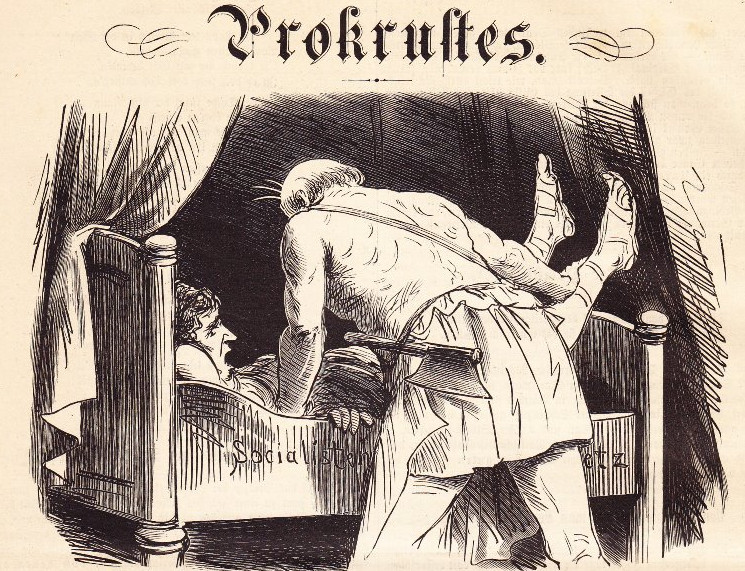
\includegraphics[scale=1.3]{images/procrustes}}
        % Start with a story.
    \end{frame}

    % Taking a step back. Going to talk about attitude determination.
    \subsection{Spacecraft Attitude Relevancy}\label{subsec:spacecraftAttitudeRelevancy}
    \begin{frame}
        \frametitle{Relevancy: Spacecraft Attitude}
        \begin{definition}
            Attitude determination = process of finding one's \textit{orientation} in space
        \end{definition} \medskip
        \begin{columns}
            \begin{column}{0.5\textwidth}
                \begin{itemize}[<+->]
                    \item Craft uses orientation to: \medskip
                    \begin{enumerate}
                        \item Orient solar panels
                        \item Direct thrusters
                        \item Position payload
                    \end{enumerate} \medskip
                    \item Uses input from: \medskip
                    \begin{enumerate}
                        \item Earth's magnetic field
                        \item Visual position of Sun
                        \item Visual position of stars
                    \end{enumerate}
                \end{itemize}
            \end{column}
            \begin{column}{0.5\textwidth}
                \centering{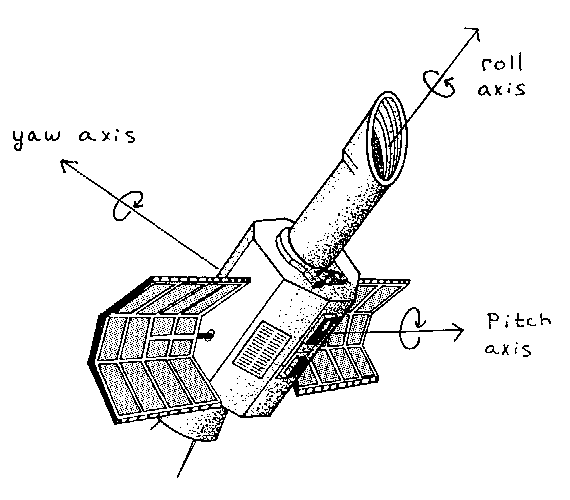
\includegraphics[scale=0.35]{images/spacecraft-attitude}}
            \end{column}
        \end{columns}
    \end{frame}

    \begin{frame}
        \frametitle{Attitude Determination}
        \begin{columns}
            \begin{column}{0.5\textwidth}
                \begin{itemize}
                    \item $R \gets$ inertial frame \bigskip
                    \item $B \gets$ body frame \bigskip
                    \item $r_i \gets$ known location in $R$ \bigskip
                    \item $b_i \gets$ observation in $B$
                \end{itemize} \bigskip
            \end{column}
            \begin{column}{0.55\textwidth}
                \centering{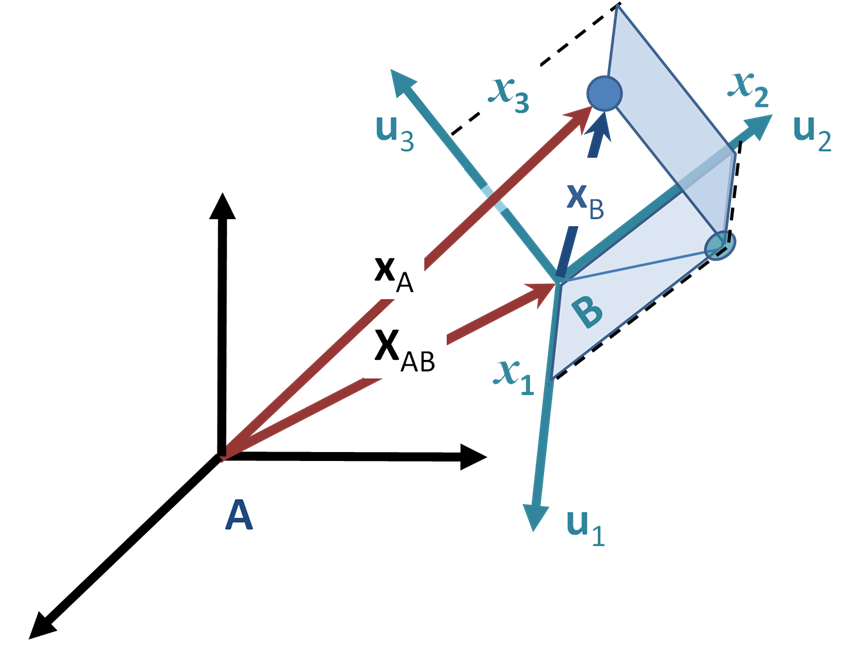
\includegraphics[scale=0.2]{images/moving-coordinate-systems.PNG}}
            \end{column}
        \end{columns} \bigskip
        \centering{\textit{Goal: Find rotation $A$ to take $R$ points to $B$}}
    \end{frame}

    \section{Rotation Representation}\label{sec:rotationRepresentation}
    \begin{frame}
        \begin{center}
            \LARGE{This begs the question\ldots what is $A$?}
        \end{center}
    \end{frame}

    \subsection{Rotation Matrices}\label{subsec:rotationMatrices}
    \begin{frame}
        \frametitle{Rotation Matrices}
        \begin{itemize}
            \item $A$ is a matrix relating $R$ to $B$ by: \pause
            \begin{equation}
                \begin{bmatrix}
                    b_1 \\
                    b_2 \\
                    b_3
                \end{bmatrix}
                =
                \begin{bmatrix}
                    A_{11} & A_{12} & A_{13} \\
                    A_{21} & A_{22} & A_{33} \\
                    A_{31} & A_{32} & A_{33}
                \end{bmatrix}
                \begin{bmatrix}
                    r_1 \\
                    r_2 \\
                    r_3
                \end{bmatrix}
                = A^{B/R}
                \begin{bmatrix}
                    r_1 \\
                    r_2 \\
                    r_3
                \end{bmatrix}
            \end{equation} \medskip \pause
            \item $A$ can also be interpreted as matrix of cosine angles:
            \begin{equation}
                A^{B/R} =
                \begin{bmatrix}
                    b_1 \cdot r_1 & b_1 \cdot r_2 & b_1 \cdot r_3 \\
                    b_2 \cdot r_1 & b_2 \cdot r_2 & b_2 \cdot r_3 \\
                    b_3 \cdot r_1 & b_3 \cdot r_2 & b_3 \cdot r_3 \\
                \end{bmatrix}
                \equiv
                \begin{bmatrix}
                    b_1 \\
                    b_2 \\
                    b_3
                \end{bmatrix}
                \cdot
                \begin{bmatrix}
                    r_1 & r_2 & r_3
                \end{bmatrix}
            \end{equation}
        \end{itemize}
    \end{frame}

    \begin{frame}
        \frametitle{Accounting for Noise in Measurement}
        \begin{itemize}[<+->]
            \item We take known location $r_i$ to measurement $b_i$ by:
            \begin{equation}
                b_i = A r_i
            \end{equation} \medskip
            \item Sensor measurements aren't perfect (sadly), we add error: \medskip
            \begin{align}
                b_i &= A r_i + v_i \\
                0 &= v_i^T A r_i
            \end{align}
        \end{itemize}
    \end{frame}

    \subsection{Quaternions}\label{subsec:quaternions}
    \begin{frame}
        \frametitle{Quaternions}
        \begin{itemize}[<+->]
            \item 3D Rotations can be represented as a 3x3 matrix, or a single 4D number \medskip
            \item The relationship between a quaternion $q$ and a direction cosine matrix $A$:
            \begin{equation}
                A =
                \begin{bmatrix}
                    1 - 2(q_2^2 + q_3^2) & 2(q_1 q_2 + q_3 q_4) & 2(q_1 q_3 + q_2 q_4) \\
                    2(q_2 q_1 + q_3 q_4) & 1-2(q_1^2+q_3^2) & 2(q_2 q_3 + q_1 q_4) \\
                    2(q_3 q_1 + q_2 q_4) & 2(q_3 q_2 + q_1 q_4) & 1 - 2(q_1^2+q_2^2)
                \end{bmatrix}
            \end{equation}
            \item Useful for low-power computing as only products are calculated
        \end{itemize}
    \end{frame}

    \section{Wahba's Problem}\label{sec:wahbasProblem}
    \begin{frame}
        \frametitle{Wahba's Problem}
        \begin{definition}
            Wahba's Problem = Finding an \textit{optimal} rotation matrix $A$ to take frame $R$ to $B$, using set of
            observations in both frames
        \end{definition} \medskip

        \begin{itemize}
            \item<2> We seek to minimize the following function:
            \begin{align}
                L(A) &= \frac{1}{2} \sum_i v_i \left\|  b_i - Ar_i \right\|^2 \\
                L(A) &= \lambda_0 - tr(AB^T)
            \end{align}
            where $\lambda_0 \equiv \sum_i v_i$ and $B \equiv \sum_i v_i b_i r_i^T$. \medskip
            \item<2> \textit{$B$ here is distinct from the spacecraft body frame $B$}
        \end{itemize}
    \end{frame}

    \begin{frame}
        \frametitle{Wahba's Problem (continued)}
        \begin{itemize}
            \item \textbf{Goal: Minimize $L(A)$}
            \begin{equation*}
                L(A) = \lambda_0 - tr(AB^T)
            \end{equation*}
            where $\lambda_0 \equiv \sum_i v_i$ and $B \equiv \sum_i v_i b_i r_i^T$. \medskip
            \item<2-> We cannot minimize $\lambda_0$, so we maximize $tr(AB^T)$\bigskip
            \item<3> This can be rewritten as the \textit{orthogonal Procrustes problem} \bigskip
            \item<3> Known approaches: SVD, TRIAD, QUEST \bigskip
        \end{itemize}
    \end{frame}

    \section{Solutions to Wahba's Problem}\label{sec:wahbasProblemSolutions}
    \subsection{SVD Method}\label{subsec:svdMethod}
    \begin{frame}
        \frametitle{SVD Method (Singular Value Decomposition)}
        \begin{itemize}[<+->]
            \item  = factorization of some matrix into three different matrices \medskip
            \item $B$ can be factored into:
            \begin{equation}
                B = U \Sigma V^T = U diag \left[ \Sigma_{11} \ \Sigma_{22} \ \Sigma_{33} \right] V^T
            \end{equation}
            % sigma contains the square roots of eigenvalues from U and V in descending order
            where $U$ and $V$ are orthogonal, and $\Sigma_{11} \geq \Sigma_{22} \geq \Sigma_{33} \geq 0$ \medskip
            \item $\Sigma$ represents diagonal matrix containing square roots of eigenvalues from $U$ or $V$ in
            descending order \medskip
            \item The optimal rotation is defined as:
            \begin{equation}
                A_{opt} = U diag \left[ 1 \ 1 \ (det U)(det V) \right] V^T
            \end{equation}
        \end{itemize}
    \end{frame}

    \subsection{QUEST Method}\label{subsec:questMethod}
    \begin{frame}
        \frametitle{QUEST Method}
        \begin{itemize}[<+->]
            \item = \textit{QUaternion ESTimator} (QUEST) \medskip
            \item The optimal rotation as a quaternion is represented as:
            \begin{equation}
                q_{opt} = \frac{1}{\sqrt{\gamma^2 + |x|^2}}
                \begin{bmatrix}
                    x \\
                    \gamma
                \end{bmatrix}
            \end{equation}
            where
            \begin{align*}
                x &\equiv \{ adj[(\lambda_{max} + trB) I - B - B^T] \} z, \\
                \gamma &\equiv det[(\lambda_{max} + trB) I - B - B^T]
            \end{align*}
        \end{itemize}
    \end{frame}

    \begin{frame}
        \frametitle{QUEST Method}
        \begin{itemize}[<+->]
            \item $\lambda_{max}$ is found
            \item = \textit{QUaternion ESTimator} (QUEST) \medskip
            \item The optimal rotation as a quaternion is represented as:
            \begin{equation}
                q_{opt} = \frac{1}{\sqrt{\gamma^2 + |x|^2}}
                \begin{bmatrix}
                    x \\
                    \gamma
                \end{bmatrix}
            \end{equation}
            where
            \begin{align*}
                x &\equiv \{ adj[(\lambda_{max} + trB) I - B - B^T] \} z, \\
                \gamma &\equiv det[(\lambda_{max} + trB) I - B - B^T]
            \end{align*}
        \end{itemize}
    \end{frame}

    \subsection{TRIAD Method}\label{subsec:triadMethod}
    \begin{frame}
        \frametitle{TRIAD Method}

    \end{frame}

    \begin{frame}
        \centering{\huge{Questions?}}
    \end{frame}
\end{document}
